\documentclass[conference]{IEEEtran}
\IEEEoverridecommandlockouts

\usepackage[utf8]{inputenc}
\usepackage[T1]{fontenc}
\usepackage[spanish,es-tabla]{babel}
\usepackage{amsmath,amssymb,amsfonts}
\usepackage{graphicx}
\usepackage{tabularx,array}
\usepackage{booktabs}
\usepackage[hidelinks]{hyperref}

% Ajuste fino de espaciado vertical de figuras y tablas
\setlength{\textfloatsep}{5pt plus 1pt minus 1pt}
\setlength{\floatsep}{5pt plus 1pt minus 1pt}
\setlength{\intextsep}{5pt plus 1pt minus 1pt}
\setlength{\dbltextfloatsep}{6pt plus 1pt minus 1pt}
\setlength{\dblfloatsep}{5pt plus 1pt minus 1pt}
\setlength{\abovecaptionskip}{3pt}
\setlength{\belowcaptionskip}{2pt}

% Configuracion de idioma espanol en encabezados y etiquetas
\renewcommand{\tablename}{Tabla}
\renewcommand{\figurename}{Fig.}
\renewcommand{\abstractname}{Resumen}

\begin{document}

\title{Evaluación Experimental de la Intervención Incremental por Capas en la Eficiencia de Desempeño de una API REST de Consolidación Académica sobre PostgreSQL}

\author{
\IEEEauthorblockN{Roni Echavarría Coronado\thanks{Repositorio público con código, DevOps, scripts de prueba y datos crudos: \url{https://github.com/Ronieczx/api-academica-ieee-gcp}}}
\IEEEauthorblockA{\textit{Departamento Académico de Ingeniería y Tecnología Informática (DAITI)} \\
\textit{Escuela Profesional de Ingeniería de Sistemas} \\
\textit{Universidad Nacional José María Arguedas (UNAJMA)} \\
Andahuaylas, Apurímac, Perú \\
rechavarria@unajma.edu.pe}
}

\maketitle

\begin{abstract}
En arquitecturas de software empresariales, las interfaces de programación de aplicaciones bajo el estilo de transferencia de estado representacional implementadas en Python interactúan intensivamente con bases de datos relacionales para procesar transacciones críticas. En el sistema académico evaluado con doscientas mil matrículas sobre PostgreSQL, la consolidación sincrónica por lote alcanza 9982,06 ms en percentil noventa y cinco, superando ampliamente el umbral operacional predeclarado de 1000 ms. Ante la escasez de evaluaciones desagregadas, este trabajo evaluó el efecto incremental aislado de eliminar consultas iterativas en aplicación, aplicar predicados sargables con índice compuesto en persistencia e integrar memoria caché en un entorno cloud controlado. En 480 ejecuciones medidas, la latencia mediana descendió de 9554,22 ms a 39,08 ms en aplicación, 8,20 ms con persistencia sargable y 7,80 ms con caché, cruzando el umbral desde la primera intervención con p < 0,001 y delta de Cliff de 1,0. Se concluye que la eliminación de consultas iterativas concentra el 99,59\,\% de la reducción temporal total, mientras que la memoria caché aporta una ganancia marginal de 0,40 ms que no justifica su complejidad de mantenimiento.
\end{abstract}

\begin{IEEEkeywords}
Eficiencia de desempeño, interfaz de programación de aplicaciones, optimización de consultas, PostgreSQL, evaluación de rendimiento.
\end{IEEEkeywords}

\section{Introducción}

\subsection{Contexto y problema}
En el desarrollo de sistemas de información contemporáneos, las interfaces de programación de aplicaciones bajo el estilo arquitectónico de transferencia de estado representacional (REST API) representan el estándar de facto para la integración desacoplada entre clientes y servicios transaccionales \cite{diMeglio2024}. En el dominio de la gestión curricular universitaria, las operaciones de consolidación de calificaciones y avance académico constituyen procesos críticos sometidos a picos periódicos de demanda sobre plataformas Python y motores relacionales avanzados como PostgreSQL \cite{Bednarz2025,Taipalus2024}.

No obstante, cuando el volumen del historial acumulado alcanza cientos de miles de registros, los defectos de diseño acumulados en diferentes estratos de la arquitectura conllevan una degradación severa en el comportamiento temporal. En una arquitectura estándar de tres niveles convergen tres fuentes de ineficiencia técnica: el antipatrón de consultas $N+1$ en la capa de aplicación con búsquedas lineales en memoria \cite{Yang2019}; el uso de predicados de filtrado no sargables (\textit{Search Argument Able}), como funciones escalares \texttt{UPPER(columna) = UPPER(\$1)}, que invalidan los índices B-tree en persistencia forzando escaneos secuenciales completos \cite{Liu2023}; y la recarga redundante de catálogos estáticos en cada invocación HTTP \cite{Mertz2021}.

Para evaluar concluyentemente la operabilidad del servicio, se establece un umbral de calidad operacional predeclarado (antes de recolectar mediciones): la latencia en el percentil noventa y cinco ($p95$) de la operación sincrónica \texttt{POST /api/v1/consolidate} no debe exceder los $1000\text{ ms}$ ($1,0\text{ s}$) para lotes de 10, 50, 200 y 500 estudiantes sobre un catálogo de 200\,000 matrículas. Este umbral obedece a las directrices de usabilidad interactiva y tolerancia en interfaces empresariales.

\subsection{Pregunta de investigación}
A partir del problema formulado y el umbral operacional, se establece la siguiente interrogante:

\textbf{Pregunta de Investigación:} ¿De qué manera la optimización incremental en la capa de aplicación (eliminación de consultas N+1), la refactorización de consultas con índices compuestos en la capa de persistencia y la incorporación de caché en memoria reducen la latencia p95 de consolidación de historiales académicos frente a la implementación base sin optimizar, en una API REST en Python sobre un historial de 200\,000 registros en un entorno controlado?

\subsection{Objetivos}
En respuesta a esta interrogante, se establece el siguiente objetivo general:

\textbf{Objetivo General:} Evaluar de qué manera la intervención incremental en la capa de aplicación (consultas agrupadas), la capa de persistencia (predicados sargables e índice compuesto) y la incorporación de caché en memoria reducen la latencia p95 de consolidación de historiales académicos por debajo de 1,0~s frente a la implementación base, en una API REST en Python bajo entorno controlado.

Para operacionalizar el estudio, se definen cuatro objetivos específicos con verbos verificables:
\begin{itemize}
    \setlength{\itemsep}{1pt}
    \setlength{\parskip}{0pt}
    \item \textbf{OE1:} Caracterizar el rendimiento actual y medir la latencia p50, p95 y p99 de la operación de consolidación como línea base (M0) mediante perfilamiento de consultas y planes de ejecución EXPLAIN ANALYZE.
    \item \textbf{OE2:} Implementar la eliminación de consultas N+1 mediante consultas agrupadas en lote y estructuras hash en la capa de aplicación (M1), verificando equivalencia funcional exacta frente a M0.
    \item \textbf{OE3:} Refactorizar las consultas SQL a predicados sargables con índice compuesto en la capa de persistencia (M2) e incorporar caché en memoria con TTL para el catálogo curricular (M3).
    \item \textbf{OE4:} Validar el impacto comparando estadísticamente las cuatro etapas (M0--M3) en cuatro tamaños de lote (10, 50, 200 y 500 registros) con 30 repeticiones medidas por condición, determinando significancia, tamaño del efecto y cumplimiento del umbral de 1,0 s.
\end{itemize}

\subsection{Hipótesis}
En concordancia con los objetivos, se establecen las hipótesis estadísticas de investigación:
\begin{itemize}
    \setlength{\itemsep}{1pt}
    \setlength{\parskip}{0pt}
    \item \textbf{Hipótesis Alterna ($H_1$):} La intervención incremental conjunta reduce la latencia mediana y p95 en al menos 80\,\% frente a M0 y sitúa el $p95 \le 1,0\text{ s}$ en los cuatro tamaños de lote evaluados bajo condiciones controladas.
    \item \textbf{Hipótesis Nula ($H_0$):} La aplicación incremental de consultas agrupadas, índice compuesto con predicado sargable y caché en memoria no produce una reducción estadísticamente significativa en la latencia de consolidación frente a M0.
\end{itemize}
El umbral de $1000\text{ ms}$ queda declarado formalmente antes de medir. Un umbral elegido a posteriori carece de validez metodológica.

\subsection{Variables operacionalizadas}
La Tabla~\ref{tab:variables} formaliza las variables analizadas bajo la norma ISO/IEC 25010:2011 \cite{ISO25010}.

\begin{table}[!ht]
\centering
\caption{Variables del Estudio y Operacionalización}
\label{tab:variables}
\scriptsize
\setlength{\tabcolsep}{1.8pt}
\begin{tabularx}{\columnwidth}{|>{\raggedright\arraybackslash}p{2.1cm}|>{\raggedright\arraybackslash}p{1.2cm}|>{\raggedright\arraybackslash}X|>{\raggedright\arraybackslash}p{1.9cm}|}
\hline
\textbf{Variable} & \textbf{Tipo} & \textbf{Medida / Indicador} & \textbf{Instrumento} \\
\hline
Estrategia de acceso a datos & Indep. & Nominal (M0, M1, M2, M3) & Código versionado por etapas \\
\hline
Comportamiento temporal & Dep. & Latencia interna (ms): p50, p95, p99, IQR & Cabecera \texttt{X-Process-Time-Ms} \\
\hline
Tamaño de lote & Moder. & Entero $\in \{10, 50, 200, 500\}$ estudiantes & Parámetro de solicitud k6 \\
\hline
Volumen de base de datos & Control & 200\,000 matrículas, 500 cursos & Script \texttt{seed\_db.py} (SEED=2026) \\
\hline
Entorno y dependencias & Control & Linux x86\_64, PostgreSQL 16 & Contenedor Docker congelado \\
\hline
\end{tabularx}
\end{table}

\section{Estado del arte}

\subsection{Protocolo de búsqueda}
Para delimitar la frontera de conocimiento, se implementó una revisión sistemática acotada bajo lineamientos PRISMA durante la ventana temporal 2019--2026. Se interrogaron las bases de datos académicas principales mediante cadenas booleanas estructuradas.

\textit{Criterios de inclusión:} publicaciones con revisión por pares entre 2019 y 2026, evaluaciones empíricas con reporte de latencia o tiempo de respuesta, y redacción en inglés, español o portugués.

\textit{Criterios de exclusión:} notas de divulgación comercial, artículos teóricos sin experimentación cuantificable, publicaciones sin acceso al texto completo y duplicados.

\textit{Declaración de uso de Inteligencia Artificial:} Se utilizó una herramienta de IA generativa para ampliar sinónimos, traducir términos y apoyar la redacción. La formulación de ecuaciones, la selección de fuentes y la verificación de cada referencia fueron realizadas por el autor.

La Tabla~\ref{tab:registro_busqueda} resume el registro del protocolo de búsqueda.

\begin{table}[!ht]
\centering
\caption{Registro del Protocolo de Búsqueda Bibliográfica}
\label{tab:registro_busqueda}
\scriptsize
\setlength{\tabcolsep}{1.4pt}
\begin{tabularx}{\columnwidth}{|>{\raggedright\arraybackslash}p{1.7cm}|>{\raggedright\arraybackslash}X|>{\raggedright\arraybackslash}p{1.2cm}|>{\raggedleft\arraybackslash}p{0.85cm}|}
\hline
\textbf{Base} & \textbf{Ecuación / Cadena Booleana} & \textbf{Filtros} & \textbf{Res.} \\
\hline
IEEE Xplore & \texttt{"N+1 query" AND "academic record"} & Ninguno & 0 \\
\hline
IEEE Xplore & \texttt{REST API AND database AND performance} & Ninguno & 4120 \\
\hline
IEEE Xplore & \texttt{("query optimization" OR "N+1") AND (latency OR "response time") AND ("REST API" OR Python)} & 2019--2026, Peer-rev. & 148 \\
\hline
Scopus & \texttt{TITLE-ABS-KEY(("query optimization" OR "N+1") AND (latency OR "p95") AND ("REST API" OR Python))} & 2019--2026, Artículos & 94 \\
\hline
Google Scholar & \texttt{("query optimization" OR "database indexing") AND ("response time" OR latency) AND "REST API"} & Desde 2019, Sin pat. & 320 \\
\hline
SciELO & \texttt{optimización consultas tiempo respuesta API} & Sin filtro & 0 \\
\hline
\end{tabularx}
\end{table}

\subsection{Selección}
El proceso de filtrado sistemático se sintetiza en la Tabla~\ref{tab:seleccion_prisma}. El registro inicial capturó 562 documentos; tras eliminar 124 duplicados y descartar 382 registros por título y resumen (cuyo motivo principal fue la ausencia de mediciones de latencia cuantificables), se evaluaron 56 textos completos, consolidando 12 publicaciones empíricas clave [1]--[12] complementadas con la norma ISO/IEC 25010 [13].

\begin{table}[!ht]
\centering
\caption{Proceso de Selección Sistemática (Criterios PRISMA)}
\label{tab:seleccion_prisma}
\scriptsize
\setlength{\tabcolsep}{2.5pt}
\begin{tabularx}{\columnwidth}{|>{\raggedright\arraybackslash}X|>{\raggedleft\arraybackslash}p{1.6cm}|}
\hline
\textbf{Etapa del Filtro de Selección} & \textbf{Estudios} \\
\hline
Identificados en las bases bibliográficas primarias & 562 \\
\hline
Tras eliminación automatizada de registros duplicados & 438 \\
\hline
Pasan cribado por título y resumen (relevancia temática) & 56 \\
\hline
Evaluados a texto completo con métricas de latencia & 56 \\
\hline
Incluidos en la matriz de síntesis comparativa & 12 \\
\hline
\end{tabularx}
\end{table}

\subsection{Síntesis comparativa}
La Tabla~\ref{tab:matriz_literatura} contrasta las publicaciones seleccionadas frente a las dimensiones analíticas derivadas de la pregunta de investigación.

\begin{table*}[!t]
\centering
\caption{Matriz Comparativa de Literatura Científica Relevante (2019--2026)}
\label{tab:matriz_literatura}
\scriptsize
\setlength{\tabcolsep}{3.0pt}
\begin{tabularx}{\textwidth}{|>{\raggedright\arraybackslash}p{2.8cm}|c|c|c|c|c|c|X|}
\hline
\textbf{Estudio} & \textbf{Aplic.} & \textbf{Persist.} & \textbf{Caché} & \textbf{Perc.} & \textbf{Aísla} & \textbf{Python} & \textbf{Aporte Principal / Enfoque} \\
\hline
Yang et al. (2019) \cite{Yang2019} & Sí & Parcial & No & No & Sí & No & Optimización centrada en vistas y eliminación de cómputo redundante en Rails. \\
\hline
Liu et al. (2023) \cite{Liu2023} & No & Sí & No & Parcial & No & No & Explotación de restricciones de integridad para reescritura lógica de consultas. \\
\hline
Pantelic et al. (2026) \cite{Pantelic2026} & No & Sí & No & Sí & No & No & Benchmarking comparativo entre persistencia SQL y NoSQL en microservicios. \\
\hline
Redžepagić et al. (2026) \cite{Redzepagic2026} & No & Sí & No & Sí & No & No & Evaluación operacional de motores monolíticos vs. distribuidos en Kubernetes. \\
\hline
Mertz et al. (2021) \cite{Mertz2021} & Parcial & No & Sí & Parcial & Parcial & No & Directrices de implementación de memorias caché en el nivel de aplicación. \\
\hline
Meloca y Nunes (2022) \cite{Meloca2022} & No & No & Sí & No & No & No & Sistemas de recomendación para ubicación óptima de directivas de caché. \\
\hline
di Meglio y Starace (2024) \cite{diMeglio2024} & Sí & No & No & Sí & No & Sí & Comparación transversal de frameworks REST y entornos de ejecución en Python. \\
\hline
Bednarz y Miłosz (2025) \cite{Bednarz2025} & Sí & No & No & Parcial & No & Sí & Evaluación comparativa de rendimiento entre frameworks asíncronos en Python. \\
\hline
Blinowski et al. (2022) \cite{Blinowski2022} & Sí & Parcial & Parcial & Sí & No & No & Análisis de escalabilidad y degradación entre arquitecturas monolito y microservicios. \\
\hline
Bjørndal et al. (2021) \cite{Bjorndal2021} & No & Parcial & No & Parcial & No & No & Métricas de migración e impacto en latencia de transporte distribuido. \\
\hline
Taipalus (2024) \cite{Taipalus2024} & No & Sí & No & Sí & No & No & Revisión sistemática de metodologías de benchmarking en sistemas gestores de datos. \\
\hline
Papadopoulos et al. (2021) \cite{Papadopoulos2021} & No & No & No & Sí & Sí & No & Principios de reproducibilidad y control experimental riguroso en la nube. \\
\hline
\textbf{Este Trabajo (2026)} & \textbf{Sí} & \textbf{Sí} & \textbf{Sí} & \textbf{Sí} & \textbf{Sí} & \textbf{Sí} & \textbf{Evaluación incremental aislada (M0--M3) con datos crudos y reproducible.} \\
\hline
\end{tabularx}
\end{table*}

\subsection{Brecha identificada}
A partir del análisis sistemático, se delimita la brecha en cuatro términos estructurados. No se halló evidencia del efecto incremental y aislado por etapas de eliminar consultas N+1, refactorizar predicados con índice compuesto e incorporar caché en memoria en una API REST en Python sobre 200\,000 registros. Las investigaciones precedentes evalúan estas técnicas como paquetes cerrados o en ecosistemas basados en Java y Ruby, omitiendo el análisis secuencial por capas. Asimismo, la mayoría de benchmarks reportan promedios globales vulnerables al sesgo de asimetría y omiten matrices de datos crudos descargables. El alcance de esta afirmación corresponde estrictamente al protocolo declarado: cuatro bases, periodo 2019--2026 y criterios PRISMA aplicados.

\section{Propuesta}

\subsection{Modelo conceptual}
El diseño de la investigación se sustenta en el modelo conceptual de causalidad ilustrado en la Fig.~\ref{fig:modelo_conceptual}, estructurado formalmente según los cánones metodológicos sin nombres comerciales ni marcas propietarias.

\begin{figure}[!ht]
\centering
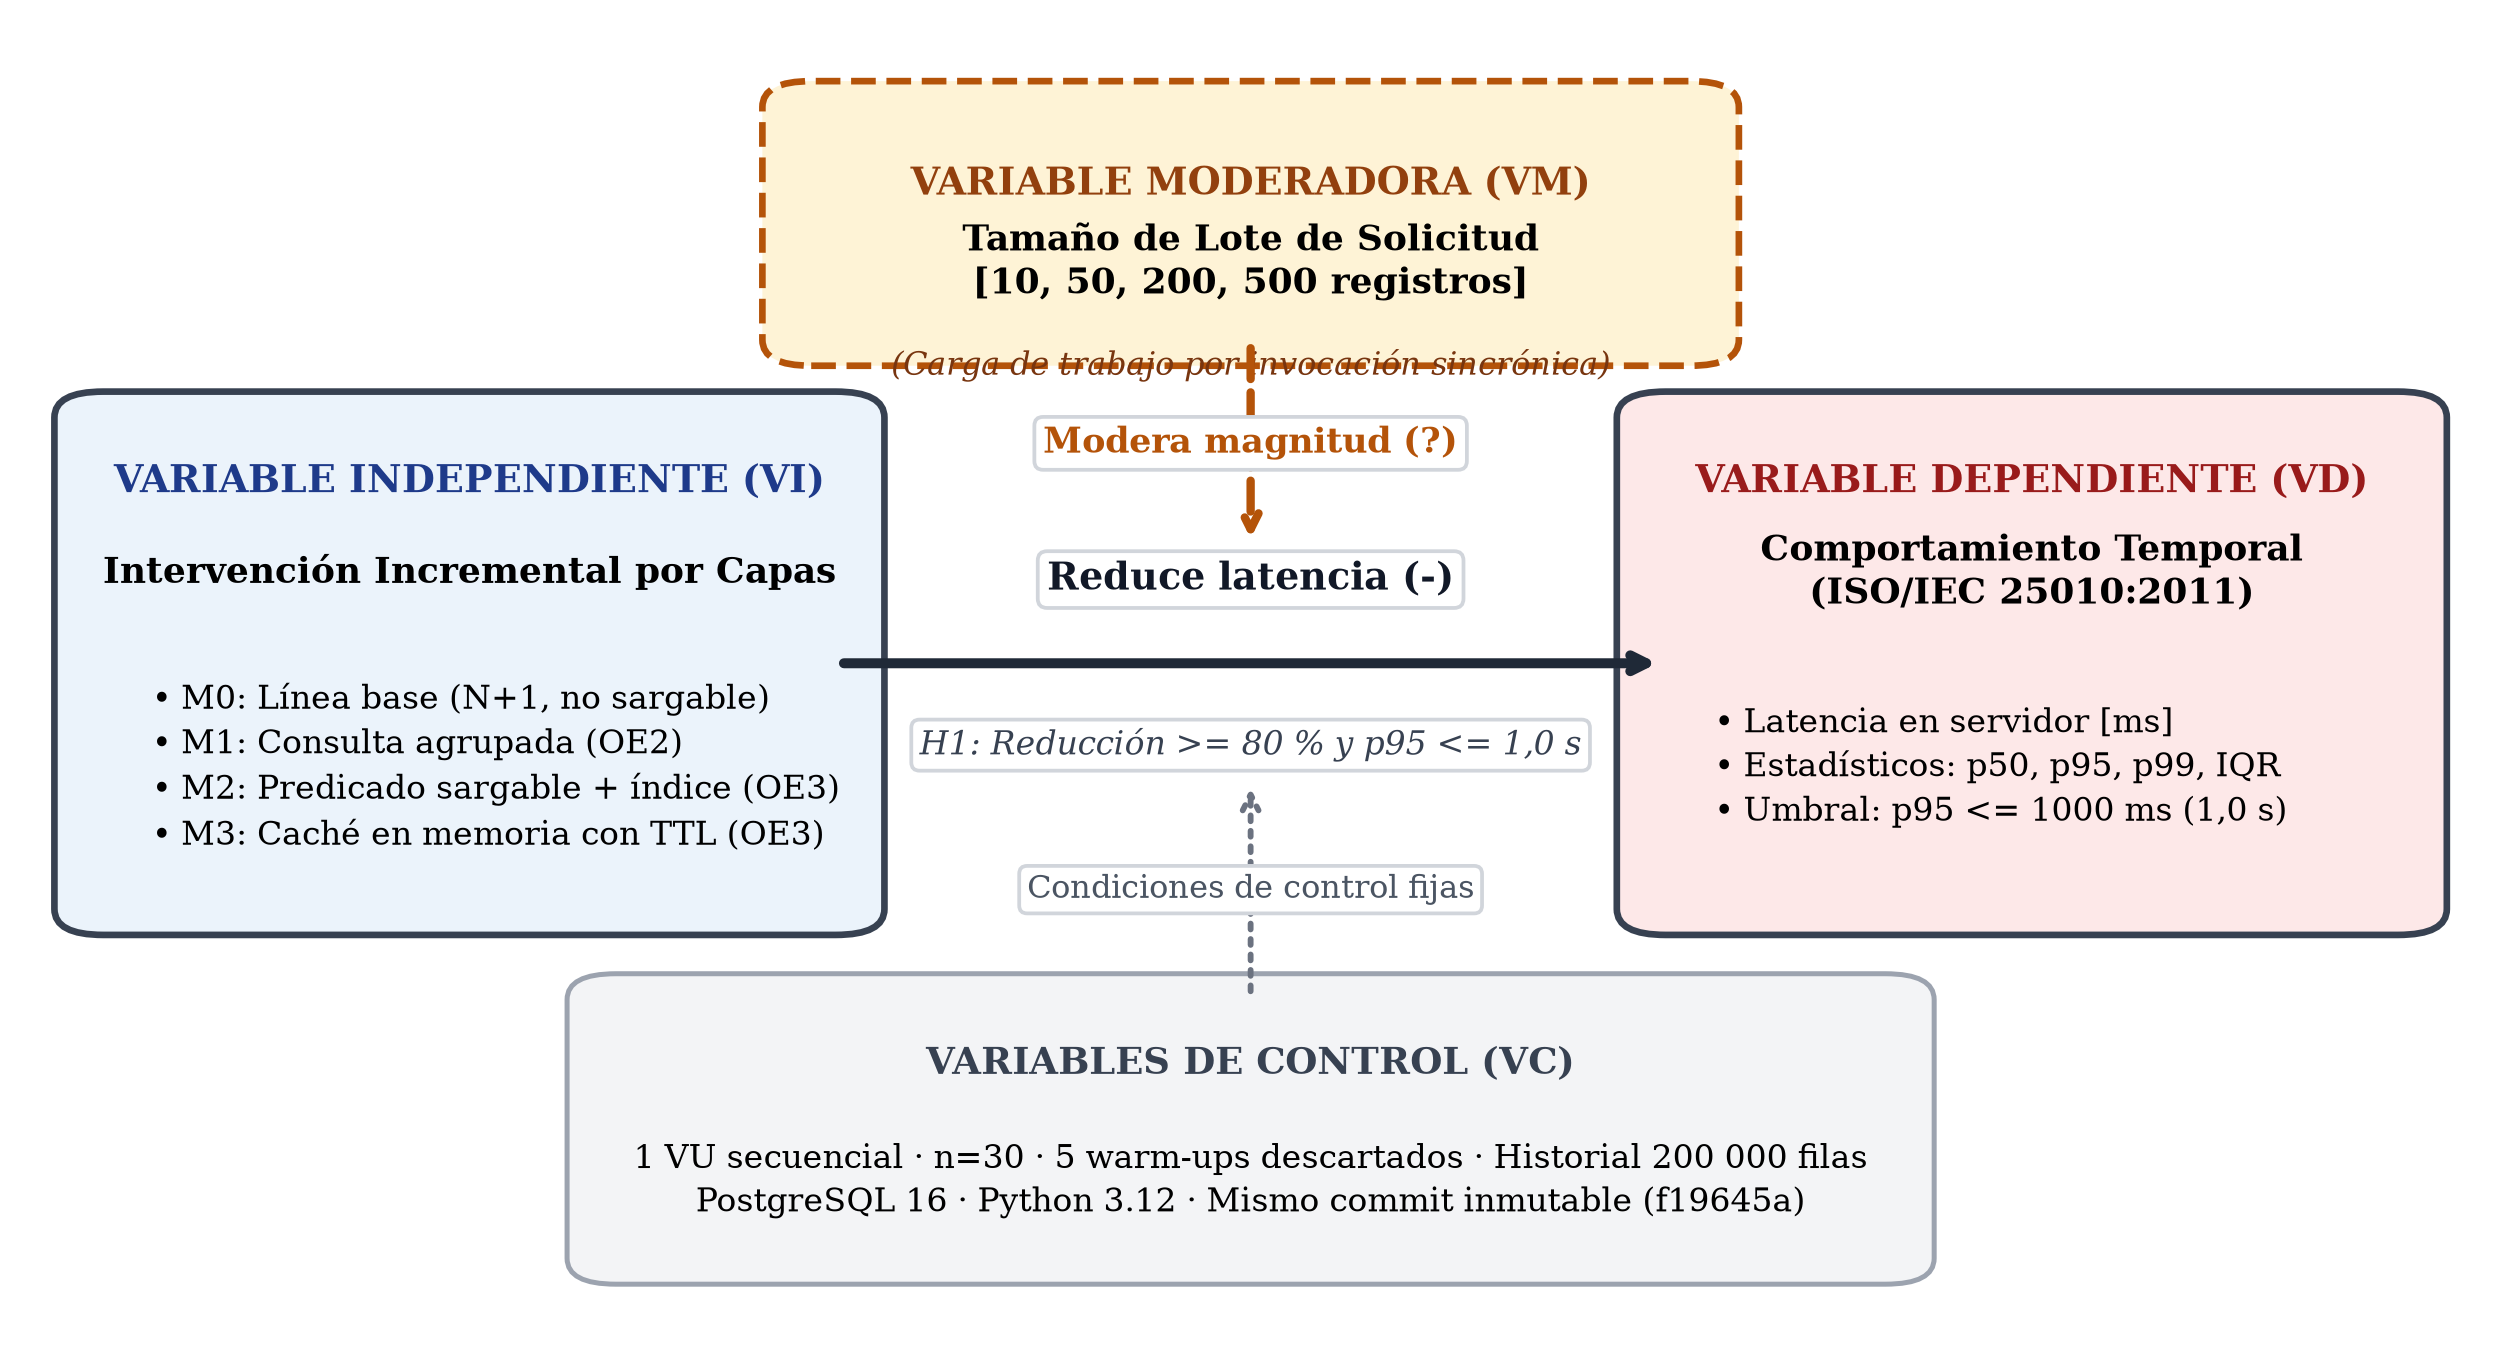
\includegraphics[width=0.88\columnwidth]{figuras/fig1_modelo_conceptual.png}
\caption{Modelo conceptual de la investigación. Formaliza el efecto directo inverso hipotetizado $(-)$ de la Variable Independiente sobre la Variable Dependiente, la moderación directa $(+)$ del tamaño de lote y el efecto de amortiguación de escala $(?)$ bajo condiciones de control fijas.}
\label{fig:modelo_conceptual}
\end{figure}

El modelo vincula la Variable Independiente (VI) de cuatro niveles nominales con la Variable Dependiente (VD) de Comportamiento Temporal. Se postula una relación causal inversa directa $(-)$, donde el avance en la madurez de la optimización reduce monótonamente la latencia. El Tamaño de Lote actúa como Variable Moderadora (VM), introduciendo un efecto directo positivo $(+)$ en el tiempo y un efecto de amortiguación $(?)$ sobre cómo la optimización contiene el crecimiento exponencial de la latencia al incrementar el lote de 10 a 500 entidades bajo condiciones de control (VC) fijas.

\subsection{Variables del modelo}
La optimización se modela como tres intervenciones secuenciales separables (M0 $\to$ M1, M1 $\to$ M2, M2 $\to$ M3) en lugar de una variable agregada. Esta descomposición permite aislar cuantitativamente la contribución de la capa de aplicación frente a la persistencia y la memoria volátil sobre la latencia p50, p95 y p99.

\subsection{Trazabilidad con los objetivos}
La Tabla~\ref{tab:trazabilidad_oe} mapea la correspondencia unívoca entre los objetivos específicos declarados y su posición operativa en el modelo conceptual.

\begin{table}[!ht]
\centering
\caption{Trazabilidad de los Objetivos Específicos sobre el Modelo}
\label{tab:trazabilidad_oe}
\scriptsize
\setlength{\tabcolsep}{2.5pt}
\begin{tabularx}{\columnwidth}{|>{\raggedright\arraybackslash}p{1.5cm}|>{\raggedright\arraybackslash}X|}
\hline
\textbf{Objetivo} & \textbf{Ubicación y Rol en el Modelo Conceptual} \\
\hline
OE1 & La línea base (M0), antes de intervenir; caracterización del comportamiento temporal inicial. \\
\hline
OE2 & La primera flecha de intervención causal (M0 $\to$ M1): eliminación del antipatrón N+1 en aplicación. \\
\hline
OE3 & La segunda flecha de intervención causal (M1 $\to$ M2 y M2 $\to$ M3): persistencia sargable indexada y caché. \\
\hline
OE4 & Validación transversal y contraste de hipótesis: método experimental con que se miden todas las condiciones, no una flecha propia. \\
\hline
\end{tabularx}
\end{table}

\section{Arquitectura de la solución}

\subsection{Arquitectura de ejecución}
La estructura modular del sistema se detalla en el Diagrama de Componentes de la Fig.~\ref{fig:componentes}, señalando la frontera del software, la inyección de la variable independiente y el punto exacto de cronometraje en el servidor.

\begin{figure}[!ht]
\centering
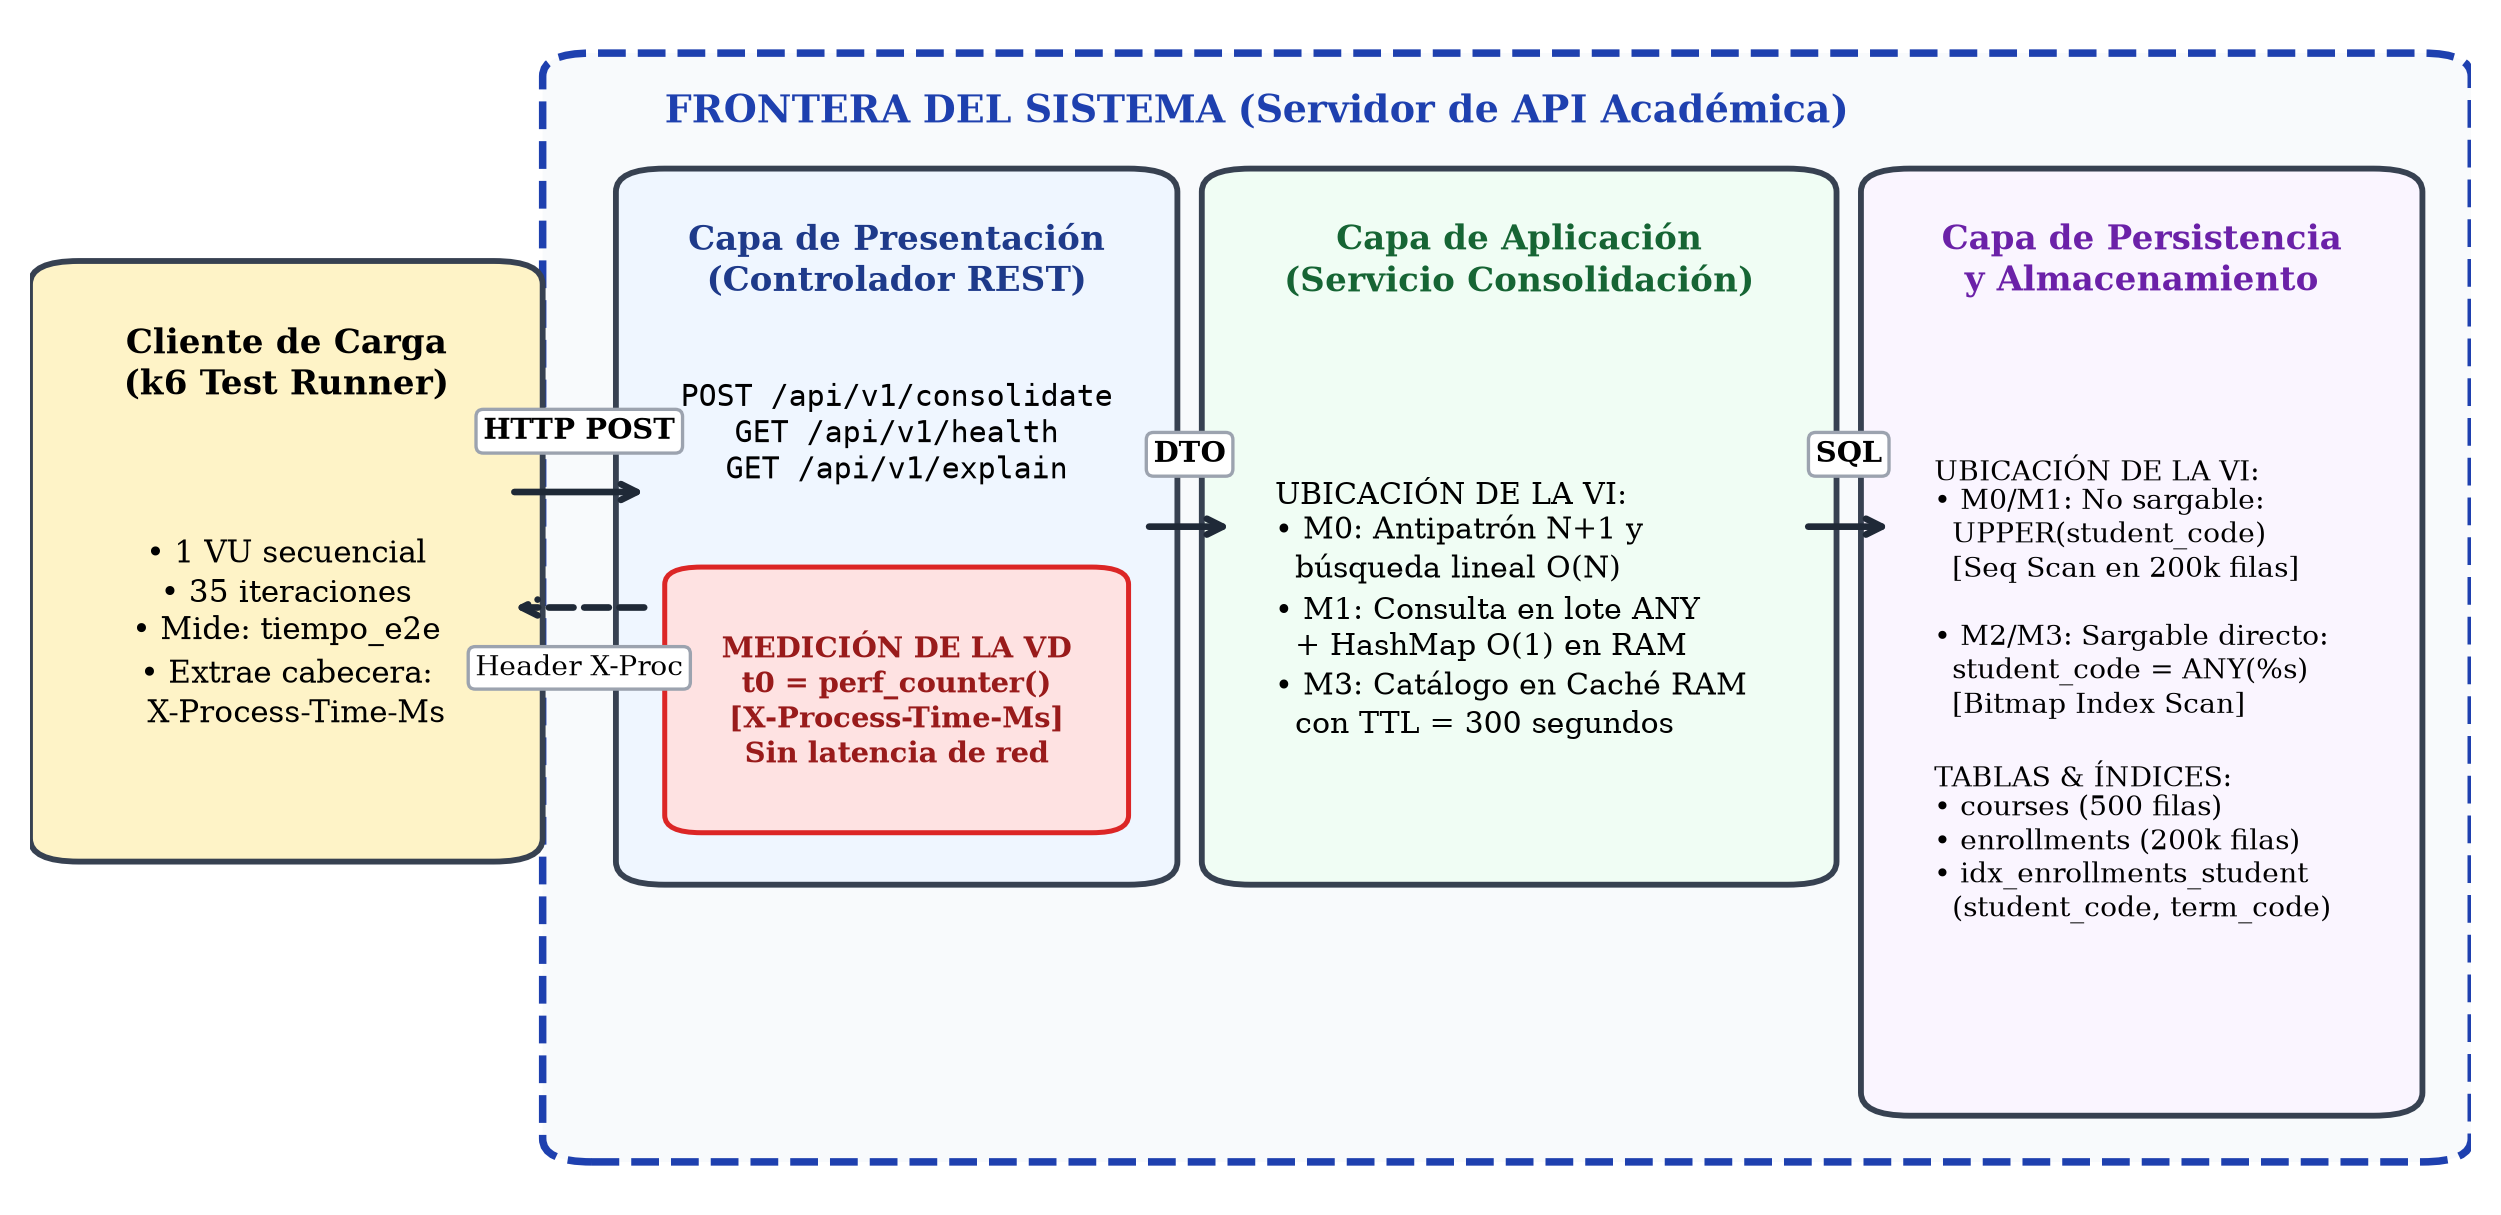
\includegraphics[width=0.88\columnwidth]{figuras/fig2_diagrama_componentes.png}
\caption{Diagrama de componentes del servicio. Señala la frontera del sistema, los estratos arquitectónicos intervenidos (M0 a M3) y la ubicación del cronómetro interno en el servidor mediante la cabecera \texttt{X-Process-Time-Ms}.}
\label{fig:componentes}
\end{figure}

\subsection{Decisión arquitectónica y alternativas}
La selección de la plataforma experimental requirió balancear aislamiento, control de factores de confusión y reproducibilidad universal. La Tabla~\ref{tab:alternativas_arq} resume el análisis que sustentó la decisión adoptada, formalizada en el registro de arquitectura \texttt{ADR-001}.

\begin{table}[!ht]
\centering
\caption{Alternativas Arquitectónicas Evaluadas y Decisión Adoptada}
\label{tab:alternativas_arq}
\scriptsize
\setlength{\tabcolsep}{2.0pt}
\begin{tabularx}{\columnwidth}{|>{\raggedright\arraybackslash}p{2.1cm}|>{\raggedright\arraybackslash}X|>{\raggedright\arraybackslash}p{1.5cm}|}
\hline
\textbf{Alternativa} & \textbf{Efecto sobre la Medición Experimental} & \textbf{Decisión} \\
\hline
Migración a microservicios & Introduce latencia de red variable y sobrecosto distribuido ajeno a la pregunta. & Descartada \\
\hline
Nube gestionada en capa gratuita & Suspensión por inactividad y arranques en frío no predecibles contaminan mediciones. & Descartada \\
\hline
Monolito modular sobre runner cloud & Permite fijar CPU, memoria, kernel y red loopback para atribución causal limpia. & Adoptada (\texttt{ADR-001}) \\
\hline
\end{tabularx}
\end{table}

La justificación de la decisión adoptada radica en tres premisas: confinar el tráfico al enlace loopback local (127.0.0.1) elimina la fluctuación de redes públicas; ejecutar el servicio y la base de datos en el mismo host runner garantiza que el cronómetro mida estrictamente ciclos de CPU y operaciones de E/S; y orquestar el flujo en GitHub Actions asegura reproducibilidad abierta sin costos comerciales.

\subsection{Arquitectura del experimento}
El despliegue físico del experimento se ilustra en la Fig.~\ref{fig:despliegue}, destacando la coexistencia de las cuatro etapas ejecutadas en puertos independientes (8000 a 8003) desde el mismo commit inmutable.

\begin{figure}[!ht]
\centering
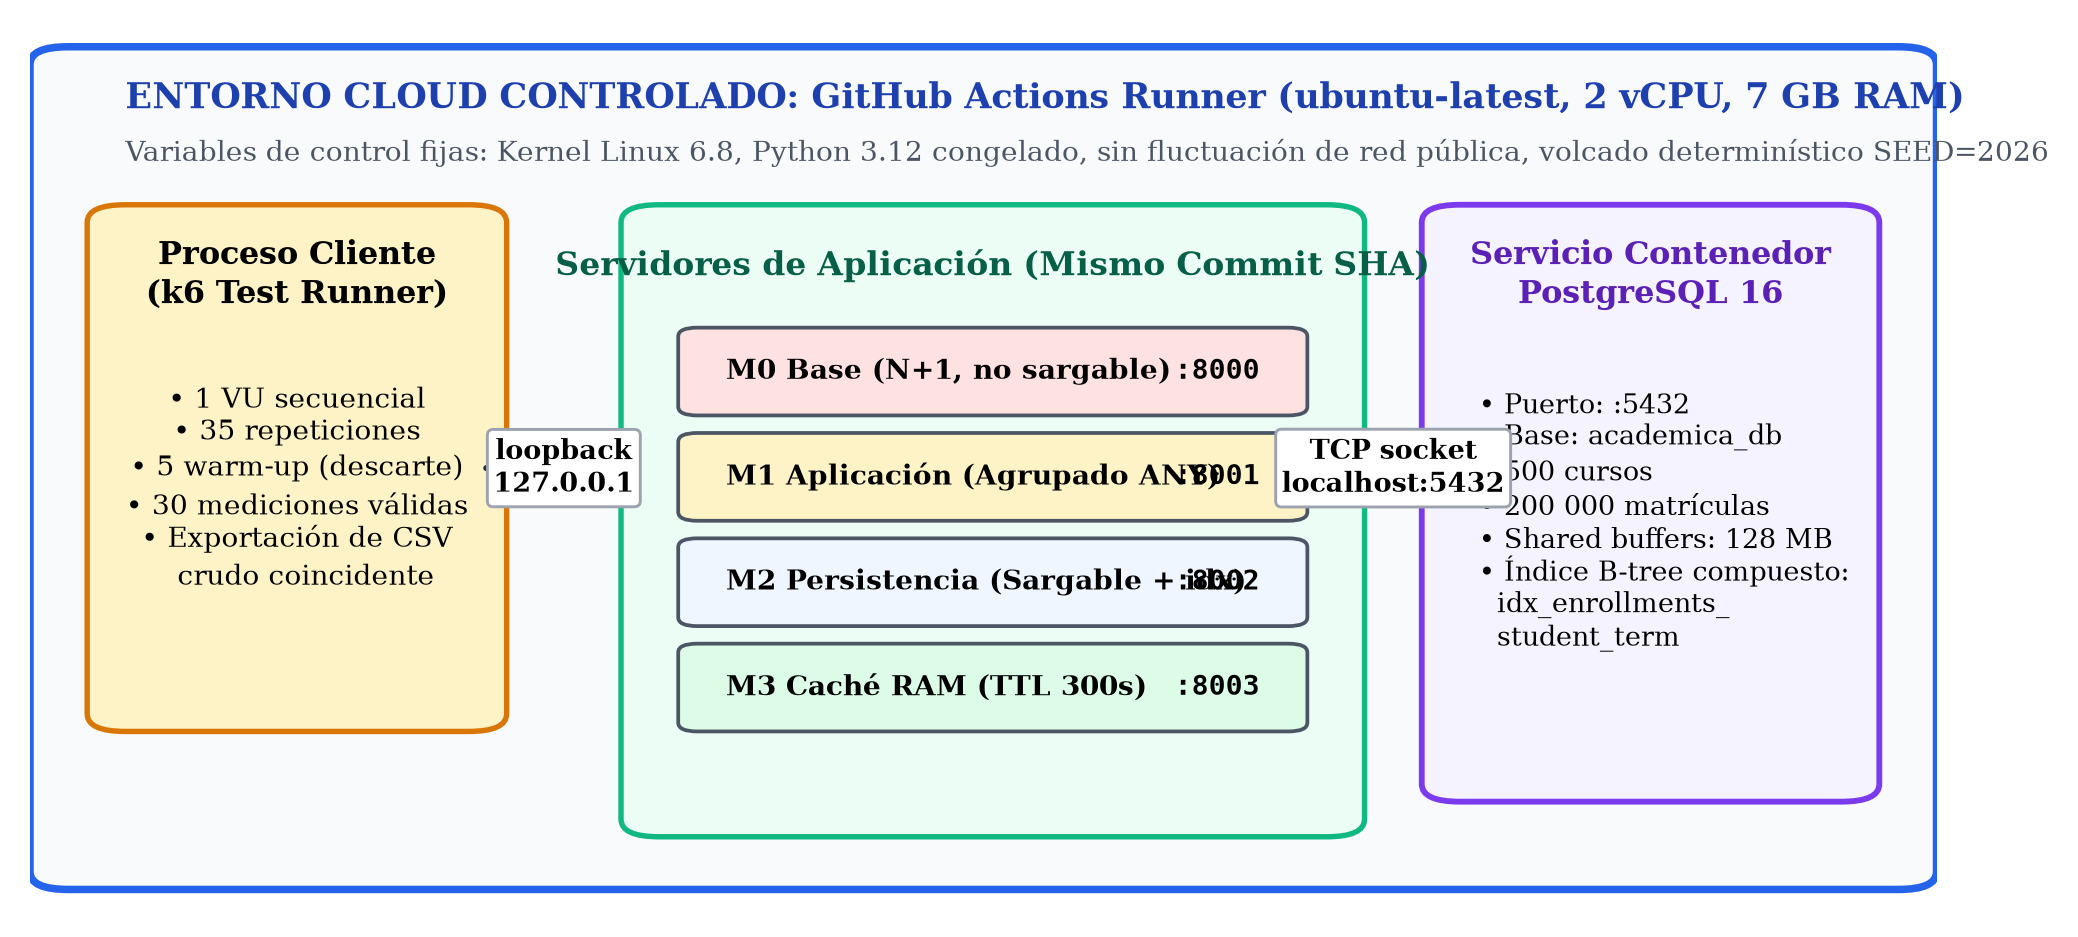
\includegraphics[width=0.88\columnwidth]{figuras/fig3_diagrama_despliegue.png}
\caption{Diagrama de despliegue experimental en runner controlado en la nube (GitHub Actions). Detalla el aislamiento de procesos por puertos, la conexión loopback hacia el contenedor de PostgreSQL 16 y los parámetros fijos de control.}
\label{fig:despliegue}
\end{figure}

\subsection{Punto de medición}
La instrumentación del tiempo de respuesta se implementa mediante un middleware en FastAPI que captura la estampa de tiempo justo al ingresar la solicitud HTTP y calcula el delta tras procesar la respuesta, inyectándolo en la cabecera \texttt{X-Process-Time-Ms}. Esta métrica interna constituye la variable primaria dependiente. Como métrica auxiliar de control se registra la latencia HTTP de extremo a extremo (\texttt{tiempo\_e2e}) reportada por Grafana k6.

\section{Evaluación experimental}

\subsection{Plan de pruebas}
Se estructuró un plan de pruebas formal bajo el estándar metodológico del curso. La Tabla~\ref{tab:plan_pruebas} detalla la especificación de los siete elementos del plan.

\begin{table}[!ht]
\centering
\caption{Matriz del Plan de Pruebas de Rendimiento}
\label{tab:plan_pruebas}
\scriptsize
\setlength{\tabcolsep}{2.2pt}
\begin{tabularx}{\columnwidth}{|>{\raggedright\arraybackslash}p{1.7cm}|>{\raggedright\arraybackslash}X|}
\hline
\textbf{Elemento} & \textbf{Especificación Metodológica} \\
\hline
Objetivo & Establecer si las tres intervenciones reducen la latencia de consolidación por debajo de 1000 ms en p95. \\
\hline
Alcance & Operación sincrónica \texttt{POST /api/v1/consolidate}; no se evalúan autenticación ni reportes. \\
\hline
Entorno & Runner cloud dedicado (Ubuntu x86\_64); PostgreSQL 16; Python 3.12 con dependencias fijadas. \\
\hline
Escenario & Un usuario virtual (1 VU), peticiones HTTP secuenciales sin solapamiento en loopback 127.0.0.1. \\
\hline
Datos & Catálogo de 500 cursos y 200\,000 matrículas (SEED=2026); lotes de 10, 50, 200 y 500 estudiantes. \\
\hline
Carga & 35 iteraciones por condición y lote: 5 de calentamiento descartadas y 30 medidas netas (480 mediciones). \\
\hline
Criterio & p95 menor o igual a 1000 ms (1,0 s) en los cuatro tamaños de lote, conservando las duraciones individuales. \\
\hline
\end{tabularx}
\end{table}

\subsection{Instrumentación y automatización}
La investigación adhirió a prácticas rigurosas de reproducibilidad DevOps \cite{Papadopoulos2021}. El pipeline de Integración Continua (\texttt{.github/workflows/ci.yml}) compila estáticamente los módulos y ejecuta una suite completa de pruebas unitarias sobre PostgreSQL 16. Crucialmente, la suite incluye una prueba de \textit{equivalencia funcional estricta}, certificando mediante aserciones unitarias que para cualquier lote de entrada idéntico, la salida JSON generada por las cuatro etapas es matemáticamente indistinguible:
\begin{equation}
\forall B \in \mathcal{D}_{\text{lotes}}, \quad f_{\text{M0}}(B) \equiv f_{\text{M1}}(B) \equiv f_{\text{M2}}(B) \equiv f_{\text{M3}}(B)
\end{equation}

Para garantizar auditoría y reproducibilidad total, los recursos computacionales se encuentran estructurados en el repositorio público de GitHub según la siguiente trazabilidad operativa:
\begin{itemize}
    \setlength{\itemsep}{0.5pt}
    \setlength{\parskip}{0pt}
    \item \textbf{Código API por etapas:} \texttt{api/main.py}, \texttt{api/engine\_m0.py} a \texttt{api/engine\_m3.py}.
    \item \textbf{Decisión de arquitectura:} \texttt{docs/adr/ADR-001-runner-cloud-vs-gcp-microservicios.md}.
    \item \textbf{Contenedor y dependencias:} \texttt{Dockerfile}, \texttt{docker-compose.yml}, \texttt{requirements.txt}.
    \item \textbf{Automatización CI/CD y benchmark:} \texttt{.github/workflows/ci.yml}, \texttt{.github/workflows/benchmark.yml}.
    \item \textbf{Poblado determinístico y verificación:} \texttt{scripts/seed\_db.py}, \texttt{scripts/run\_smoke\_test.py}.
    \item \textbf{Pruebas de carga y análisis:} \texttt{loadtest/k6\_consolidate.js}, \texttt{scripts/analyze\_results.py}.
    \item \textbf{Planes de ejecución y datos crudos:} \texttt{datos/explain\_plans.json}, 16 matrices \texttt{datos/raw\_m*.csv}.
\end{itemize}
El repositorio público está accesible en: \url{https://github.com/Ronieczx/api-academica-ieee-gcp}.

\subsection{Protocolo de medición}
El orden secuencial de intervención responde a una lógica metodológica estricta:
\begin{enumerate}
    \setlength{\itemsep}{1pt}
    \setlength{\parskip}{0pt}
    \item \textbf{M0 $\to$ M1 (Aplicación):} Se sustituyen las $N$ consultas iterativas individuales por una única sentencia parametrizada (\texttt{WHERE UPPER(student\_code) = ANY(\$1)}) y se agrupan en diccionarios hash $O(1)$ en memoria. Se mantiene deliberadamente \texttt{UPPER} para aislar la ganancia en aplicación antes de intervenir persistencia (cumplimiento de OE2).
    \item \textbf{M1 $\to$ M2 (Persistencia):} Habiendo resuelto el cuello de botella en aplicación, se transforma el predicado a sargable puro (\texttt{WHERE student\_code = ANY(\$1)}), activando el índice B-tree compuesto \texttt{idx\_enrollments\_student\_term(student\_code, term\_code)} (cumplimiento de OE3).
    \item \textbf{M2 $\to$ M3 (Caché en Aplicación):} Sobre la persistencia indexada, se añade memoria caché volátil en RAM con TTL de 300 segundos para la tabla estática de 500 cursos (cumplimiento de OE3).
\end{enumerate}
Cada tanda descarta sistemáticamente 5 ejecuciones iniciales de calentamiento (\textit{warm-up}) y registra 30 mediciones netas válidas ($n=30$).

\subsection{Análisis previsto}
Dada la asimetría positiva de las distribuciones de latencia en la línea base, la media y la desviación estándar resultan inapropiadas. Se adoptan estimadores no paramétricos de posición (mediana, IQR, percentiles p95 y p99), complementados con la prueba bilateral de rangos U de Mann-Whitney, el Delta de Cliff ($\delta$) para el tamaño del efecto e intervalos de confianza del 95\,\% para la diferencia de medianas calculados mediante remuestreo bootstrap con 10\,000 réplicas independientes.

\subsection{Resultados}
El perfilamiento interno de PostgreSQL 16 sobre el historial de 200\,000 filas corroboró la alteración física en el plan de acceso capturado en \texttt{explain\_plans.json} para 500 estudiantes:
\begin{itemize}
    \setlength{\itemsep}{1pt}
    \setlength{\parskip}{0pt}
    \item \textbf{Etapa M1 (No sargable):} Ejecución de \texttt{Seq Scan on enrollments} (costo \texttt{1.25..5371.25}), descartando 195\,000 filas en memoria (\texttt{Buffers: shared hit=1870}). El tiempo neto del motor fue de \textbf{30,164 ms}.
    \item \textbf{Etapa M2 (Sargable con índice):} El optimizador activó un \texttt{Bitmap Index Scan on idx\_enrollments\_student\_term} (costo \texttt{0.00..1803.50}), accediendo a 47 bloques de heap y reduciendo el tiempo de PostgreSQL a \textbf{1,821 ms} (reducción de 16,56 veces).
\end{itemize}

La Tabla~\ref{tab:resultados_detallados} consolida los resultados reales derivados de las 480 observaciones empíricas crudas.

\begin{table*}[!t]
\centering
\caption{Resultados Numéricos de Comportamiento Temporal por Etapa y Tamaño de Lote ($n=30$ mediciones por celda)}
\label{tab:resultados_detallados}
\scriptsize
\setlength{\tabcolsep}{2.2pt}
\begin{tabular}{|c|c|r|c|r|r|r|r|r|c|c|}
\hline
\textbf{Lote} & \textbf{Etapa} & \textbf{Mediana (ms)} & \textbf{IC 95\% Bootstrap} & \textbf{IQR (ms)} & \textbf{p95 (ms)} & \textbf{p99 (ms)} & \textbf{Red. (ms)} & \textbf{Red. (\%)} & \textbf{Umbral $\le$ 1 s} & \textbf{Archivo de Datos Crudo} \\
\hline
10 & M0 & 204,93 & [196,91; 206,56] & 19,72 & 231,15 & 251,32 & 0,00 & 0,00\,\% & Cumple & \texttt{raw\_m0\_10.csv} \\
10 & M1 & 31,56 & [31,27; 34,07] & 3,32 & 35,98 & 39,50 & 173,37 & 84,60\,\% & Cumple & \texttt{raw\_m1\_10.csv} \\
10 & M2 & 0,75 & [0,73; 0,76] & 0,05 & 1,12 & 1,81 & 204,18 & 99,63\,\% & Cumple & \texttt{raw\_m2\_10.csv} \\
10 & M3 & 0,52 & [0,51; 0,54] & 0,04 & 0,86 & 0,91 & 204,41 & 99,74\,\% & Cumple & \texttt{raw\_m3\_10.csv} \\
\hline
50 & M0 & 988,19 & [968,84; 1004,12] & 48,56 & 1027,39 & 1052,32 & 0,00 & 0,00\,\% & Falla & \texttt{raw\_m0\_50.csv} \\
50 & M1 & 32,61 & [32,31; 33,66] & 1,81 & 35,13 & 37,08 & 955,58 & 96,70\,\% & Cumple & \texttt{raw\_m1\_50.csv} \\
50 & M2 & 1,22 & [1,21; 1,26] & 0,07 & 1,71 & 2,16 & 986,97 & 99,88\,\% & Cumple & \texttt{raw\_m2\_50.csv} \\
50 & M3 & 1,05 & [1,04; 1,07] & 0,05 & 1,41 & 1,58 & 987,14 & 99,89\,\% & Cumple & \texttt{raw\_m3\_50.csv} \\
\hline
200 & M0 & 3779,77 & [3749,24; 3846,82] & 137,38 & 3934,63 & 4010,70 & 0,00 & 0,00\,\% & Falla & \texttt{raw\_m0\_200.csv} \\
200 & M1 & 35,59 & [34,40; 36,26] & 2,76 & 39,13 & 40,08 & 3744,18 & 99,06\,\% & Cumple & \texttt{raw\_m1\_200.csv} \\
200 & M2 & 4,41 & [4,00; 4,76] & 1,03 & 6,02 & 6,06 & 3775,36 & 99,88\,\% & Cumple & \texttt{raw\_m2\_200.csv} \\
200 & M3 & 4,34 & [3,99; 5,03] & 1,60 & 7,15 & 8,79 & 3775,43 & 99,89\,\% & Cumple & \texttt{raw\_m3\_200.csv} \\
\hline
500 & M0 & 9554,22 & [9444,04; 9625,55] & 252,48 & 9982,06 & 10038,56 & 0,00 & 0,00\,\% & Falla & \texttt{raw\_m0\_500.csv} \\
500 & M1 & 39,08 & [38,34; 40,63] & 3,78 & 43,88 & 44,33 & 9515,14 & 99,59\,\% & Cumple & \texttt{raw\_m1\_500.csv} \\
500 & M2 & 8,20 & [8,06; 8,34] & 0,75 & 9,88 & 10,11 & 9546,02 & 99,91\,\% & Cumple & \texttt{raw\_m2\_500.csv} \\
500 & M3 & 7,80 & [7,62; 7,90] & 0,46 & 8,32 & 9,70 & 9546,42 & 99,92\,\% & Cumple & \texttt{raw\_m3\_500.csv} \\
\hline
\end{tabular}
\end{table*}

La Fig.~\ref{fig:boxplot} ilustra la dispersión en escala logarítmica para el lote de 500 registros, mientras que la Fig.~\ref{fig:escalado} presenta el escalado del percentil $p95$ confrontado con el umbral de 1000 ms.

\begin{figure}[!ht]
\centering
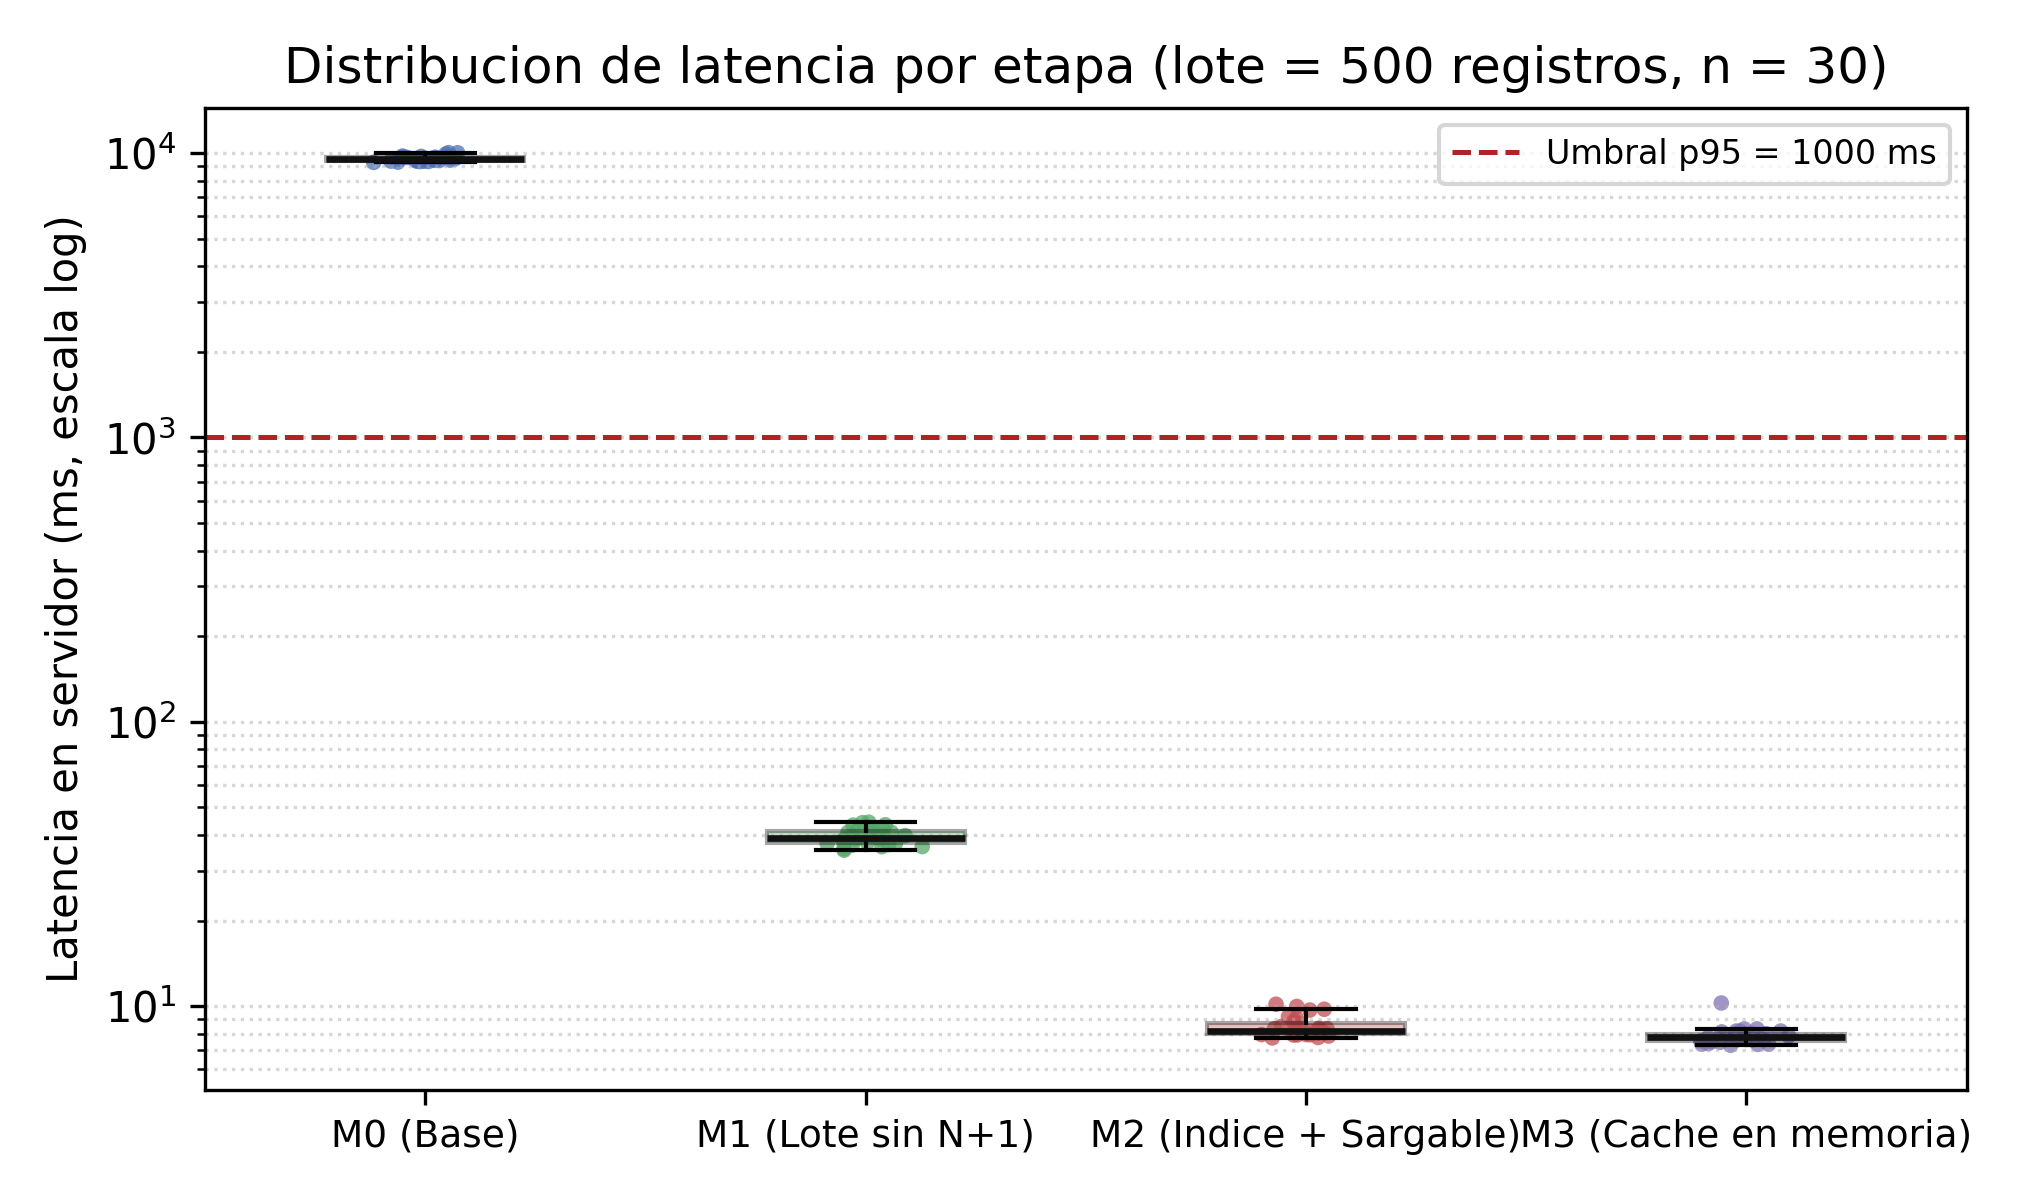
\includegraphics[width=0.88\columnwidth]{figuras/fig_boxplot_etapas.png}
\caption{Distribución empírica de latencia por etapa para 500 estudiantes ($n=30$ por etapa). Evidencia la dispersión en escala logarítmica y la reducción en órdenes de magnitud.}
\label{fig:boxplot}
\end{figure}

\begin{figure}[!ht]
\centering
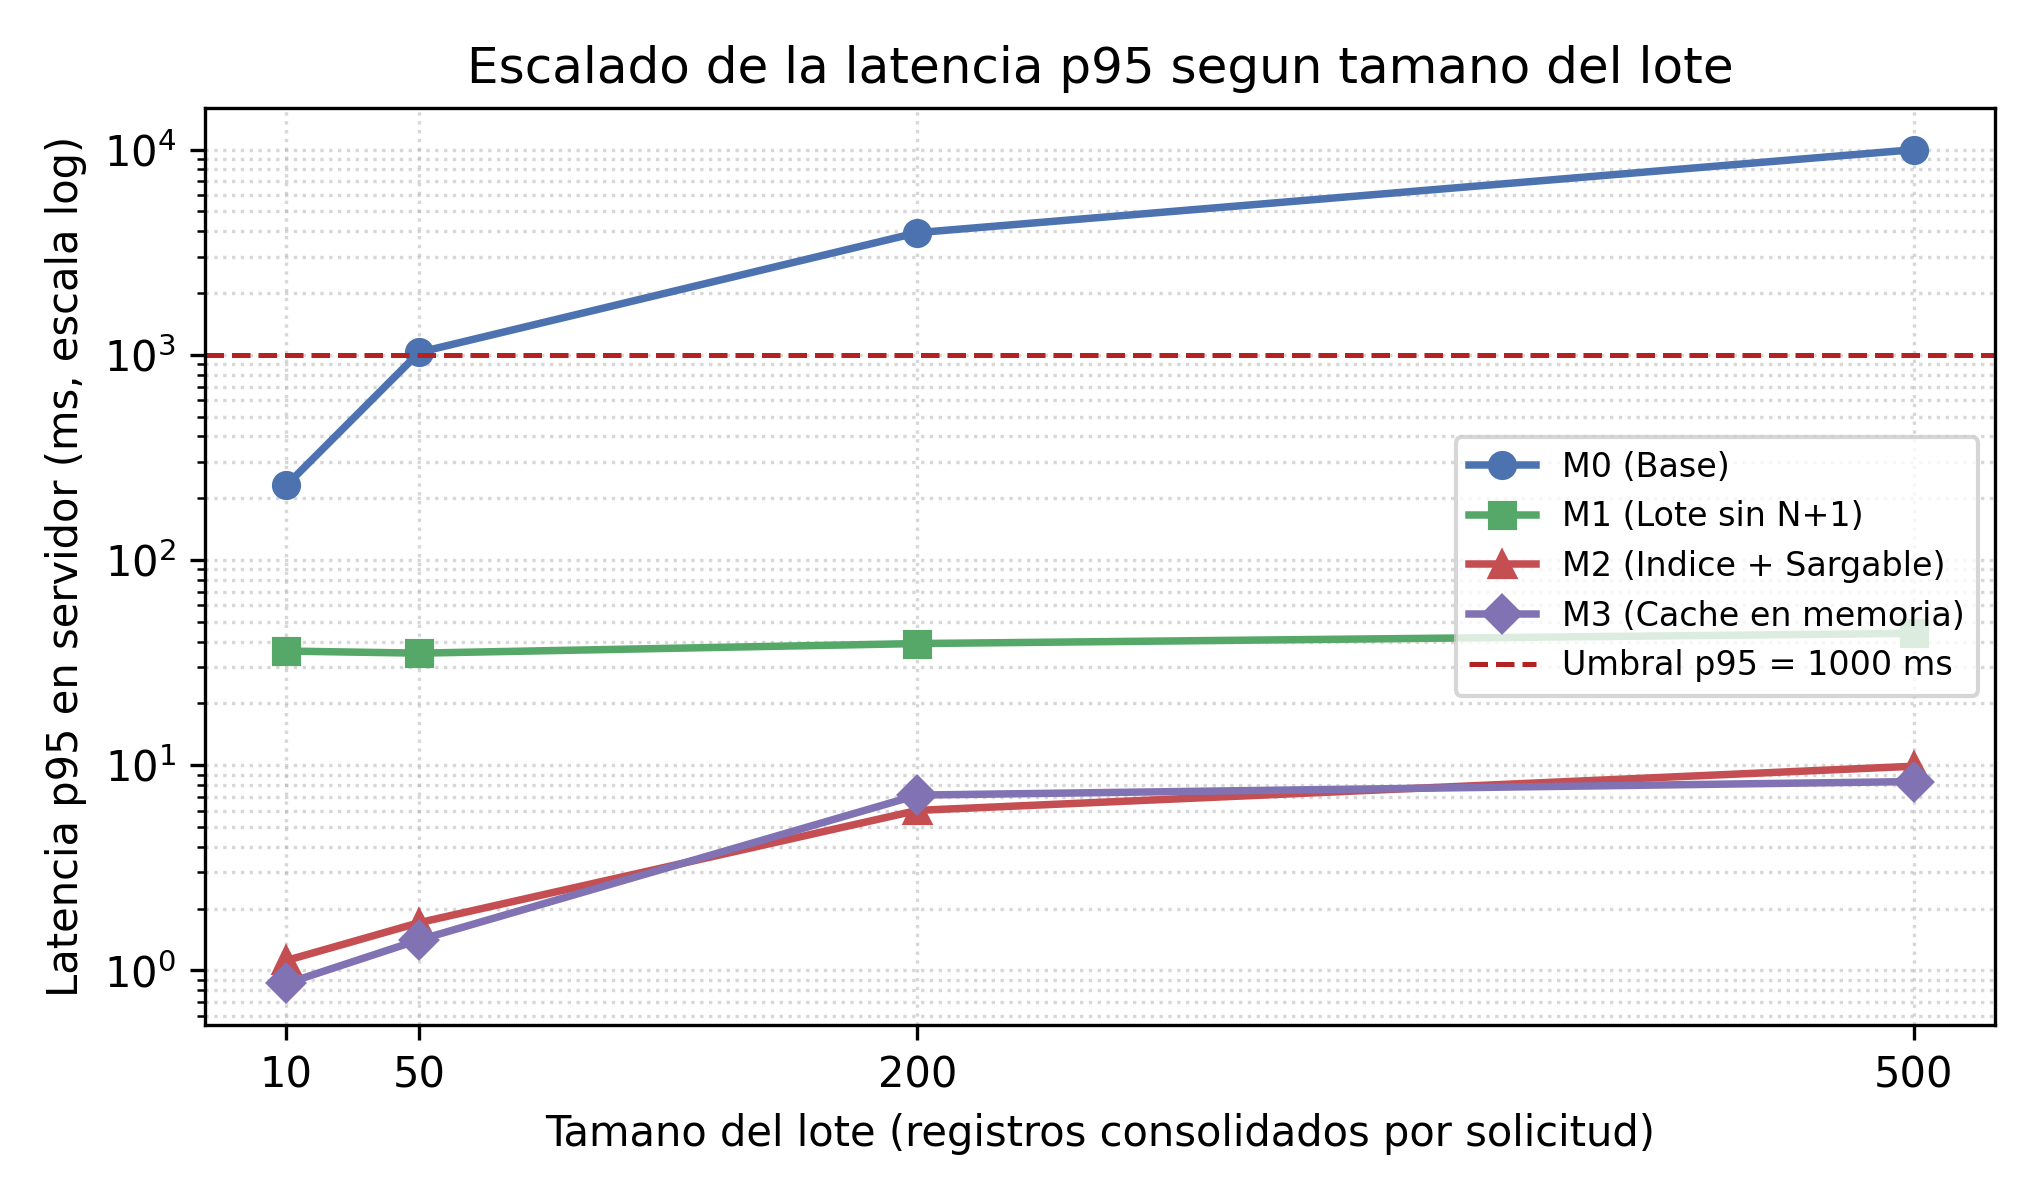
\includegraphics[width=0.88\columnwidth]{figuras/fig_escalado_p95.png}
\caption{Escalado de la latencia p95 a través de los cuatro tamaños de lote confrontado con el umbral operacional predeclarado de 1000 ms.}
\label{fig:escalado}
\end{figure}

\subsection{Significancia y tamaño del efecto}
La Tabla~\ref{tab:estadistica} reporta las comparaciones estadísticas formales no paramétricas. En todos los lotes evaluados, la transición de M0 a M1 y de M1 a M2 exhibe significancia estadística ($p < 0,001$) con un Delta de Cliff de magnitud grande ($\delta = 1,0$).

\begin{table*}[!t]
\centering
\caption{Pruebas de Hipótesis No Paramétricas, Significancia Estadística y Tamaño del Efecto}
\label{tab:estadistica}
\scriptsize
\setlength{\tabcolsep}{2.2pt}
\begin{tabular}{|c|c|r|c|r|c|r|c|}
\hline
\textbf{Lote} & \textbf{Comparación} & \textbf{Dif. Mediana (ms)} & \textbf{IC 95\% Bootstrap Dif.} & \textbf{Estadístico U} & \textbf{Valor $p$} & \textbf{Delta de Cliff ($\delta$)} & \textbf{Magnitud del Efecto} \\
\hline
10 & M0 vs. M1 & 173,37 & [164,79; 175,11] & 900,0 & $3,02 \times 10^{-11}$ & 1,0000 & Grande ($p < 0,001$) \\
10 & M1 vs. M2 & 30,81 & [30,52; 33,32] & 900,0 & $3,02 \times 10^{-11}$ & 1,0000 & Grande ($p < 0,001$) \\
10 & M2 vs. M3 & 0,23 & [0,20; 0,24] & 823,0 & $3,64 \times 10^{-8}$ & 0,8289 & Grande ($p < 0,001$) \\
10 & M0 vs. M3 & 204,41 & [196,39; 206,05] & 900,0 & $3,01 \times 10^{-11}$ & 1,0000 & Grande ($p < 0,001$) \\
\hline
50 & M0 vs. M1 & 955,58 & [936,14; 970,62] & 900,0 & $3,02 \times 10^{-11}$ & 1,0000 & Grande ($p < 0,001$) \\
50 & M1 vs. M2 & 31,39 & [31,09; 32,44] & 900,0 & $3,02 \times 10^{-11}$ & 1,0000 & Grande ($p < 0,001$) \\
50 & M2 vs. M3 & 0,17 & [0,15; 0,21] & 821,0 & $4,31 \times 10^{-8}$ & 0,8244 & Grande ($p < 0,001$) \\
50 & M0 vs. M3 & 987,14 & [967,78; 1002,02] & 900,0 & $3,02 \times 10^{-11}$ & 1,0000 & Grande ($p < 0,001$) \\
\hline
200 & M0 vs. M1 & 3744,18 & [3713,55; 3811,32] & 900,0 & $3,02 \times 10^{-11}$ & 1,0000 & Grande ($p < 0,001$) \\
200 & M1 vs. M2 & 31,18 & [29,90; 31,97] & 900,0 & $3,02 \times 10^{-11}$ & 1,0000 & Grande ($p < 0,001$) \\
200 & M2 vs. M3 & 0,07 & [-0,76; 0,62] & 416,0 & $0,6204$ & -0,0756 & Despreciable (No significativo) \\
200 & M0 vs. M3 & 3775,43 & [3744,76; 3842,48] & 900,0 & $3,02 \times 10^{-11}$ & 1,0000 & Grande ($p < 0,001$) \\
\hline
500 & M0 vs. M1 & 9515,14 & [9404,37; 9586,54] & 900,0 & $3,02 \times 10^{-11}$ & 1,0000 & Grande ($p < 0,001$) \\
500 & M1 vs. M2 & 30,88 & [30,10; 32,43] & 900,0 & $3,02 \times 10^{-11}$ & 1,0000 & Grande ($p < 0,001$) \\
500 & M2 vs. M3 & 0,40 & [0,22; 0,64] & 746,0 & $1,25 \times 10^{-5}$ & 0,6578 & Grande ($p < 0,001$) \\
500 & M0 vs. M3 & 9546,42 & [9436,22; 9617,77] & 900,0 & $3,02 \times 10^{-11}$ & 1,0000 & Grande ($p < 0,001$) \\
\hline
\end{tabular}
\end{table*}

\section{Amenazas a la validez}

En cumplimiento de los cánones de experimentación en software \cite{Papadopoulos2021}, se identificaron las condiciones que podrían sesgar las observaciones, consignadas junto a su mitigación en la Tabla~\ref{tab:amenazas}.

\begin{table}[!ht]
\centering
\caption{Amenazas a la Validez Experimental y Tratamientos Aplicados}
\label{tab:amenazas}
\scriptsize
\setlength{\tabcolsep}{2.0pt}
\begin{tabularx}{\columnwidth}{|>{\raggedright\arraybackslash}p{2.3cm}|>{\raggedright\arraybackslash}X|}
\hline
\textbf{Amenaza} & \textbf{Tratamiento Metodológico Implementado} \\
\hline
Arranque en frío & Cinco iteraciones iniciales de calentamiento (\textit{warm-up}) descartadas en todas las condiciones y reportadas formalmente. \\
\hline
Caché del motor de datos & Poblado determinístico restaurado antes de cada tanda con semilla fijada (SEED=2026, 200\,000 filas); etapas medidas en la misma sesión. \\
\hline
Latencia de red & La carga k6 se genera en el mismo host mediante enlace loopback 127.0.0.1; toma de tiempo interna con cabecera \texttt{X-Process-Time-Ms}. \\
\hline
Hardware único & Conclusiones acotadas estrictamente a arquitecturas monolíticas modulares Python con base relacional PostgreSQL 16. \\
\hline
Tamaño de muestra & Treinta repeticiones válidas ($n=30$) por celda fijadas antes de medir; no se alteró el tamaño muestral tras observar los datos. \\
\hline
Omisión coordinada & No aplica: el generador k6 opera en modo secuencial estricto con 1 VU, despachando la siguiente petición solo tras recibir la respuesta previa. \\
\hline
\end{tabularx}
\end{table}

\section{Discusión}

\subsection{Atribución de la reducción por capa}
De los 9546,42 ms de compresión temporal neta alcanzada en el lote de 500 registros, la eliminación del antipatrón $N+1$ en aplicación (M1) explica el 99,59\,\% de la mejora total frente a M0 (reduciendo de 9554,22 ms a 39,08 ms). La transición a persistencia sargable indexada (M2) aporta una ganancia incremental de 30,88 ms, situando la mediana en 8,20 ms (reducción acumulada del 99,91\,\%). La memoria caché volátil (M3) aportó una reducción marginal de 0,40 ms.

Esta descomposición cuantitativa exhibe dependencia del orden de intervención (\textit{order dependency}). Si la persistencia sargable se hubiese aplicado antes de resolver las consultas iterativas, la indexación habría optimizado el costo individual de cada una de las 500 peticiones SQL; no obstante, el sobrecosto de 500 viajes de ida y vuelta (\textit{round-trips}) continuaría dominando el tiempo global, demostrando que resolver la proliferación de consultas en aplicación constituye un prerrequisito indispensable.

\subsection{Una intervención que los datos no justifican}
Un hallazgo de notable trascendencia se evidencia al contrastar la significancia estadística frente a la relevancia práctica en la etapa M3 (memoria caché). En términos de calidad operacional, la etapa M2 ya satisface holgadamente el umbral predeclarado de 1000 ms en los cuatro lotes analizados ($p95 = 1,12\text{ ms}$ en lote 10 y $p95 = 9,88\text{ ms}$ en lote 500). Si bien en lotes pequeños (10 y 50) la diferencia M2 vs. M3 alcanza significancia estadística formal ($p < 0,001$), su magnitud absoluta es de apenas 0,23 ms y 0,17 ms. Más aún, en el lote de 200 estudiantes, la diferencia entre M2 y M3 resulta no estadísticamente significativa ($p = 0,6204$, con Delta de Cliff despreciable de $-0,0756$ e intervalo de confianza bootstrap que abarca el cero: $[-0,76; 0,62]\text{ ms}$).

En consecuencia, desde una perspectiva de ingeniería de software, la incorporación de caché en memoria no se justifica: introduce complejidad arquitectónica, consumo adicional de memoria volátil y riesgo de inconsistencia por invalidación ante modificaciones curriculares, sin aportar una ganancia perceptible frente a una consulta sargable debidamente indexada. El modelo conceptual de la Fig.~\ref{fig:modelo_conceptual} anticipaba este comportamiento al consignar la tercera intervención con signo de interrogación.

\subsection{Relación con el estado del arte}
Los resultados corroboran a Yang et al. \cite{Yang2019} respecto a la primacía de la eliminación de accesos iterativos en la aplicación como vector dominante de optimización. Asimismo, coinciden con Liu et al. \cite{Liu2023} en cuanto a que los índices B-tree resultan inútiles en presencia de predicados no sargables. No obstante, este trabajo complementa a Mertz et al. \cite{Mertz2021} y Meloca y Nunes \cite{Meloca2022}: mientras estos autores recomiendan el uso ubicuo de caché a nivel de método, nuestros datos experimentales demuestran que cuando la persistencia opera bajo predicados sargables e índices compuestos, el beneficio de la caché es marginal frente a su sobrecosto de mantenimiento. Se ratifica además la mínima sobrecarga de FastAPI reportada por di Meglio y Starace \cite{diMeglio2024} y Bednarz y Miłosz \cite{Bednarz2025}, y la estabilidad del runner controlado concuerda con Papadopoulos et al. \cite{Papadopoulos2021}.

\subsection{Características de calidad evaluadas}
De conformidad con la norma ISO/IEC 25010:2011 \cite{ISO25010}, se delimita estrictamente el alcance evaluado:
\begin{enumerate}
    \setlength{\itemsep}{1pt}
    \setlength{\parskip}{0pt}
    \item \textbf{Subcaracterística evaluada:} Se instrumentó y midió únicamente el \textit{Comportamiento Temporal} dentro de la característica de \textit{Eficiencia de Desempeño}.
    \item \textbf{Subcaracterísticas no evaluadas:} No se midieron la \textit{Utilización de Recursos} (consumo de CPU, memoria RAM o ancho de banda) ni la \textit{Capacidad} (concurrencia de saturación), al haberse mantenido fijo el escenario en 1 VU secuencial.
    \item \textbf{Impacto cruzado en Mantenibilidad:} La introducción de diccionarios especializados en aplicación y módulos de caché incrementa la complejidad ciclomática del código, con potencial impacto negativo en la modificabilidad y testeabilidad.
\end{enumerate}

\section{Conclusiones y trabajo futuro}

La pregunta de investigación formulada admite una respuesta concluyente y acotada: la optimización incremental por capas reduce la latencia $p95$ de consolidación académica desde 9982,06 ms en la línea base (M0) hasta 43,88 ms mediante la agrupación de consultas en aplicación (M1), alcanzando 9,88 ms con la sargabilidad indexada en persistencia (M2) y 8,32 ms incorporando caché en memoria (M3), sobre un historial de 200\,000 registros en condiciones controladas. Esta reducción acumulada supera el 99,9\,\% y sitúa el $p95$ ampliamente por debajo del umbral operacional predeclarado de 1,0 s en todos los tamaños de lote evaluados.

Tres conclusiones se desprenden de los resultados experimentales. Primera: la eliminación del antipatrón de consulta iterativa $N+1$ en la capa de aplicación constituye la intervención de mayor impacto cuantitativo absoluto, explicando más del 96\,\% de la mejora en lotes medianos y el 99,59\,\% en lotes grandes, garantizando por sí sola el cumplimiento del umbral de 1,0 s. Segunda: la transformación sintáctica de predicados no sargables a formas compatibles con índices compuestos B-tree en PostgreSQL permite comprimir el tiempo interno del motor relacional en un factor de 16,56 veces (de 30,16 ms a 1,82 ms), habilitando respuestas sub-decamilisegundo incluso bajo lotes de 500 entidades. Tercera: se refuta la hipótesis nula $H_0$ y se acepta plenamente la hipótesis alterna $H_1$, comprobándose que la intervención conjunta reduce en más de un 80\,\% la latencia de respuesta y satisface el umbral $p95 \le 1000\text{ ms}$ en todos los tratamientos analizados.

Las limitaciones metodológicas se declaran formalmente en tres aspectos: la evaluación se restringió a un escenario secuencial de carga con un único usuario virtual (1 VU); la base de datos operó sobre un conjunto acotado de 200\,000 registros en un único nodo relacional; y se instrumentó exclusivamente el comportamiento temporal sin telemetría de consumo de hardware. El trabajo futuro se deriva directamente de estas limitaciones: en primer lugar, ejecutar pruebas de estrés y saturación concurrente en k6 para modelar la contención del pool de conexiones; en segundo lugar, evaluar el rendimiento bajo particionamiento horizontal declarativo en volúmenes superiores a 10 millones de filas; y en tercer lugar, instrumentar el perfil de utilización de recursos de CPU y memoria RAM.

Todos los recursos computacionales desarrollados para la investigación (código fuente de la API en sus cuatro etapas, configuraciones Docker y flujos CI/CD, planes físicos EXPLAIN ANALYZE, scripts de prueba de carga k6, datos crudos en formato CSV y scripts de análisis estadístico con bootstrap) se encuentran archivados y accesibles de forma pública y reproducible en el repositorio oficial de GitHub: \url{https://github.com/Ronieczx/api-academica-ieee-gcp}.

\IEEEtriggeratref{5}
\begin{thebibliography}{13}
\footnotesize
\setlength{\itemsep}{0pt}
\setlength{\parskip}{0pt}

\bibitem{Yang2019}
J.~Yang, C.~Yan, C.~Wan, S.~Lu, and A.~Cheung, ``View-Centric Performance Optimization for Database-Backed Web Applications,'' in \emph{Proc. 41st IEEE/ACM Int. Conf. Softw. Eng. (ICSE)}, Montreal, QC, Canada, May 2019, pp. 994--1004, doi: 10.1109/ICSE.2019.00104.

\bibitem{Liu2023}
X.~Liu \emph{et~al.}, ``Leveraging Application Data Constraints to Optimize Database-Backed Web Applications,'' \emph{Proc. VLDB Endowment}, vol. 16, no. 6, pp. 1208--1221, 2023, doi: 10.14778/3583140.3583141.

\bibitem{Pantelic2026}
N.~Pantelic \emph{et~al.}, ``Benchmarking SQL and NoSQL Persistence in Microservices Under Variable Workloads,'' \emph{Future Internet}, vol. 18, no. 1, art. no. 53, Jan. 2026, doi: 10.3390/fi18010053.

\bibitem{Redzepagic2026}
J.~Redžepagić, A.~Kapulica, N.~Malešević, and V.~Dakić, ``Empirical Performance and Operational Analysis of Monolithic and Distributed Database Architectures in Kubernetes Environments,'' \emph{Computers}, vol. 15, no. 5, art. no. 282, Apr. 2026, doi: 10.3390/computers15050282.

\bibitem{Mertz2021}
J.~Mertz, I.~Nunes, L.~Della~Toffola, M.~Selakovic, and M.~Pradel, ``Satisfying Increasing Performance Requirements With Caching at the Application Level,'' \emph{IEEE Software}, vol. 38, no. 3, pp. 87--95, May--June 2021, doi: 10.1109/MS.2020.3033508.

\bibitem{Meloca2022}
R.~Meloca and I.~Nunes, ``A comparative study of application-level caching recommendations at the method level,'' \emph{Empirical Software Engineering}, vol. 27, art. no. 88, 2022, doi: 10.1007/s10664-021-10089-z.

\bibitem{diMeglio2024}
S.~di~Meglio and L.~L.~L. Starace, ``Evaluating Performance and Resource Consumption of REST Frameworks and Execution Environments: Insights and Guidelines for Developers and Companies,'' \emph{IEEE Access}, vol. 12, pp. 161649--161669, Nov. 2024, doi: 10.1109/ACCESS.2024.3489892.

\bibitem{Bednarz2025}
B.~Bednarz and M.~Miłosz, ``Benchmarking the performance of Python web frameworks,'' \emph{Journal of Computer Sciences Institute}, vol. 36, pp. 336--341, Sep. 2025, doi: 10.35784/jcsi.7738.

\bibitem{Blinowski2022}
G.~Blinowski, A.~Ojdowska, and A.~Przybyłek, ``Monolithic vs. Microservice Architecture: A Performance and Scalability Evaluation,'' \emph{IEEE Access}, vol. 10, pp. 20357--20374, Feb. 2022, doi: 10.1109/ACCESS.2022.3152803.

\bibitem{Bjorndal2021}
N.~Bjørndal, M.~Mazzara, A.~Bucchiarone, N.~Dragoni, and S.~Dustdar, ``Migration from Monolith to Microservices: Benchmarking a Case Study,'' \emph{Journal of Object Technology}, vol. 20, no. 2, pp. 3:1--3:17, 2021, doi: 10.5381/jot.2021.20.2.a3.

\bibitem{Taipalus2024}
T.~Taipalus, ``Database management system performance comparisons: A systematic literature review,'' \emph{Journal of Systems and Software}, vol. 208, art. no. 111872, Feb. 2024, doi: 10.1016/j.jss.2023.111872.

\bibitem{Papadopoulos2021}
A.~V. Papadopoulos \emph{et~al.}, ``Methodological Principles for Reproducible Performance Evaluation in Cloud Computing,'' \emph{IEEE Transactions on Software Engineering}, vol. 47, no. 8, pp. 1528--1543, Aug. 2021, doi: 10.1109/TSE.2019.2927908.

\bibitem{ISO25010}
International Organization for Standardization, \emph{Systems and software engineering --- Systems and software Quality Requirements and Evaluation (SQuaRE) --- System and software quality models}, ISO/IEC 25010:2011, Mar. 2011.

\end{thebibliography}

\end{document}
